\chapter{Obtención de geometría}

En este capítulo se presenta la reconstrucción tridimensional automática de una superficie utilizando técnicas computacionales.
Se introducen distintos métodos que permiten la construcción automática de modelos, discutiendo sus características según propiedades de la superficie a representar y tecnologías utilizadas.
La construcción del modelo se presenta en dos etapas. Inicialmente se obtiene una nube de puntos correspondiente a la superficie utilizando técnicas y dispositivos para este propósito para luego procesar la información obtenida y construir una malla tridimensional. Mediante este procesamiento se obtiene información adicional como grupos de puntos que representan caras de una malla y las normales que identifican la orientación de la superficie. 

\section{Obtención de la nube de puntos}

En esta sección se estudian los fundamentos matemáticos, técnicas y dispositivos relacionados al problema de la correspondencia de puntos de la realidad con puntos bidimensionales en el plano imagen, obtenido por una cámara, y la posterior determinación de su profundidad.

\subsection{Correspondencia}

%Al calcular coordenadas tridimensionales a partir de imágenes obtenidas por capturas de video se introducen errores propios del modelo (modelo \emph{pinhole}, modelo imaginario que utiliza una cámara) por ello es necesario hacer una corrección obteniendo una correspondencia entre el modelo real y el ideal. El objetivo del proceso de calibración es obtener dicha correspondencia. Luego de la calibración las coordenadas obtenidas son en dos dimensiones y corresponden a la proyección sobre el plano imagen. Para completar las coordenadas tridimensionales en el modelo es necesario calcular la profundidad de cada punto. Es con este fin que se utiliza el método de triangulación.

%El modelo ideal que se utiliza en las cámaras es el modelo \emph{pinhole}\cite{LibroCompGrafica3}, el que se describe a continuación para un caso básico.

Una cámara, por medio de una proyección central, establece una correspondencia entre puntos del espacio con puntos bidimensionales en su plano imagen. En particular se estudiará el modelo de camara pinhole.
%ponemos que es el mas simple?

Se considera el centro de proyección $C$, tambien centro óptico de la cámara, como el origen de un sistema de coordenadas Euclideano, y $Z = f$ el plano de la imagen o plano focal.

\begin{figure}[H]
  \centering
    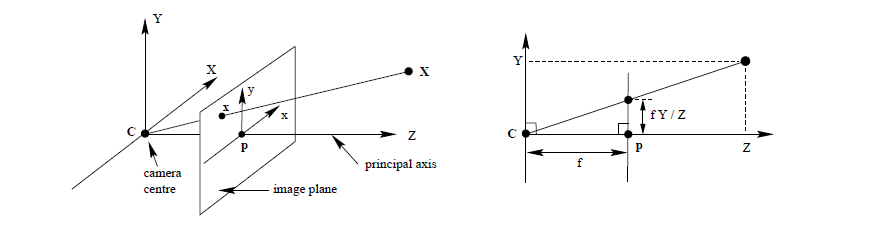
\includegraphics[width=0.8\textwidth]{./Cap6_reconstruccion/pinhole.png}
  \caption{Geometría de cámara \emph{pinhole}. $C$ es centro de la cámara y $p$ el punto principal}
  \label{fig:Calib-Pinhole}
\end{figure}

Un punto en el espacio $A=(A_X, A_Y, A_Z)^T$ se corresponde con el punto $a$ en el plano imagen, dado por la intersección del rayo que pasa por el centro de cámara y el punto $A$ con el plano imagen. El punto $A$ se corresponde con $(\frac{fA_X}{A_Z}, \frac{fA_Y}{A_Z}, f)^T$ en el plano imagen considerando que el centro de coordenadas del plano imagen coincide con el punto principal $P$.

Considerando la representación de los puntos como vectores homogéneos se expresa la proyección central como una correspondencia lineal entre las coordenadas homogéneas.

\[
\begin{pmatrix}
A_X \\ A_Y \\ A_Z \\ 1
\end{pmatrix}
\to
\begin{pmatrix}
fA_X \\ fA_Y \\ A_Z
\end{pmatrix}
=
\begin{pmatrix}
f & 0 & 0 & 0 \\
0 & f & 0 & 0 \\
0 & 0 & 1 & 0 \\
\end{pmatrix}
\begin{pmatrix}
A_X \\ A_Y \\ A_Z \\ 1
\end{pmatrix}
\]

Dado $A_h = (A_X,A_Y,A_Z,1)^T$ y la proyección $a$ sobre el plano imagen, la correspondencia utilizando el método pinhole es:
$a=PA_h$

Siendo
\[
P = 
\begin{pmatrix}
f & 0 & 0 & 0 \\
0 & f & 0 & 0 \\
0 & 0 & 1 & 0 \\
\end{pmatrix}
\]

\subsection{Método de triangulación}
Este método determina las coordenadas $(x,y,z)$ de un punto utilizando la posición bidimensional dada por las perspectivas de dos proyecciones de las que se conocen los centros de perspectiva y planos de proyección\cite{PresUnivYonsei}.

Escena con dos dimensiones:

\begin{figure}[H]
  \centering
    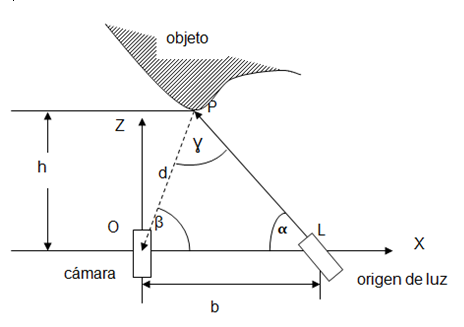
\includegraphics[width=0.65\textwidth]{./Cap6_reconstruccion/triangulacion.PNG}
  \caption{Diagrama con propiedades trigonométricas para escena 2D.}
  \label{fig:Triangulacion}
\end{figure}

Este método tiene como objetivo calcular la distancia $d$ de la cámara al punto $P$ a partir de los ángulos $\alpha$, $\beta$ y la distancia $b$ entre el proyector y la cámara.
El ángulo $\alpha$ y la distancia $b$ son dados por la calibración de la escena.
El ángulo $\beta$ esta dado por la geometría de la proyección.

\[
\left.
\begin{array}{l}
\frac{d}{\sin (\alpha)} = \frac{b}{\sin (\gamma)} 	\\
\gamma = \pi - (\alpha + \beta)						\\
\sin (\pi - \gamma) = \sin (\gamma)
\end{array}
\right \rbrace
\frac{d}{\sin(\alpha)} = \frac{b}{\sin(p - \gamma)} = \frac{b}{\sin(\alpha + \beta)} \Rightarrow d = b . \frac{\sin(\alpha)}{\sin(\alpha + \beta)}
\]

Las coordenadas cartesianas quedan determinadas por:
\[
X_o = d. \cos (\beta)
\]
\[
Z_o = d. \sin (\beta) = h
\]

Escena con tres dimensiones:

\begin{figure}[H]
  \centering
    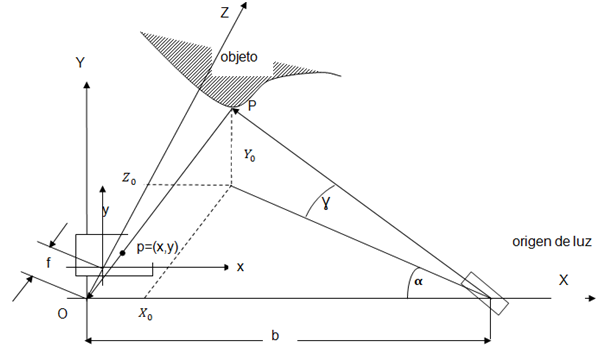
\includegraphics[width=0.65\textwidth]{./Cap6_reconstruccion/triangulacion-2.PNG}
  \caption{Diagrama con propiedades trigonométricas para escena 3D.}
  \label{fig:Triangulacion2}
\end{figure}

Se asume $Z = f$ siendo $f$ el plano en el cuál se proyecta el punto $P(X_o, Y_o, Z_o)$, obteniendo como resultado de la proyección el punto $p(x,y)$.
El centro óptico del proyector está situado en el eje $X$.
Se considera realizada una pre-calibración en la cual se define:
\[
P = (x,y), \quad \frac{X_o}{x} = \frac{Z_o}{f} = \frac{Y_o}{y} = k \to (k * x,k * y,k * f)
\]
Por trigonometría:
\[
\tan (\alpha) = \frac{Z_0}{(b - X_0)} \Rightarrow Z_0 = \tan (\alpha) (b - X_0) \quad 
\]
\[
k * f = \tan (\alpha)(b - k * x)
\]
\[
k (f + x * \tan (\alpha)) = b * \tan (\alpha)
\]
\[
k = \frac	{b * \tan (\alpha)}{f + x * \tan (\alpha)}
\]
\[
X_o = \frac{x * b * \tan (\alpha)}{f + x * \tan (\alpha)}, \quad Yo = \frac{y * b * \tan (\alpha)}{f + x * \tan (\alpha)},\quad Zo = \frac{f * b * \tan (\alpha)}{f + x * \tan (\alpha)}
\]


Los métodos que resuelven obtener la geometría de una escena tridimensional sin tener contacto físico se pueden clasificar como activos o pasivos\footnote{IEEE TRANSACTION ON PATTERN ANALYSIS AND MACHINE INTELIGENCE, VOL. PAMI-5, NO.2 MARCH 1983. A Perspective on Range Finding Techniques for Computer Vision.}.
Los métodos pasivos son aquellos en los que no es necesario utilizar luz adicional a la luz ambiente.
%los activos?%

\subsection{Visión estéreo}

Visión estéreo es un método pasivo para obtener la estructura tridimensional de una escena. Se utiliza el método de triangulación sin intervención de luz auxiliar y la correspondencia es establecida entre dos o más imágenes.
Los algoritmos que utilizan este método están clasificados basados en diferencias de la geometría de la imagen, en las estrategias para resolver la correspondencia entre puntos y en las diferentes estructuras computacionales utilizadas\cite{StereoReview}.
Se realiza un preproceso de las imágenes para identificar las principales características que se utilizarán. Luego, se define qué tipo de correspondencia se utilizará.
La principal desventaja de este método es que en caso de oclusión, hay regiones que no tienen correspondencia en las dos imágenes, por lo tanto no se puede establecer la correspondencia de puntos.
Las variantes que influyen en la geometría de la imagen son, ejes ópticos\footnote{Ejes ópticos.} paralelos o no, paradigma binocular o multiocular.
%referenciar%
La correspondencia entre una o más vistas de la escena se puede realizar basada en distintas estrategias que son \emph{separate area} o \emph{features}.
\begin{itemize}
   \item \emph{separate area}: basada en correlación del brillo e intensidad. Se utilizan patrones de brillo aplicados a un \emph{pixel} y sus vecinos utilizando principio de localidad. Las diferencias en la perspectiva de la imagen o cambios en luminosidad absoluta de la escena pueden generar errores.
   \item \emph{features}: las características usadas para la correspondencia son aristas, puntos o segmentos dadas por cambios de intensidad de la imagen. Esta estrategia es más estable ante la variación de luminosidad absoluta y en la práctica la correspondencia es más rápida.
\end{itemize}
La disposición de la geometría en visión estéreo incluye un par de cámaras y los ejes ópticos son paralelos entre sí y perpendiculares a la línea base que es dada por los dos centros ópticos de las cámaras.

\begin{figure}[H]
  \centering
    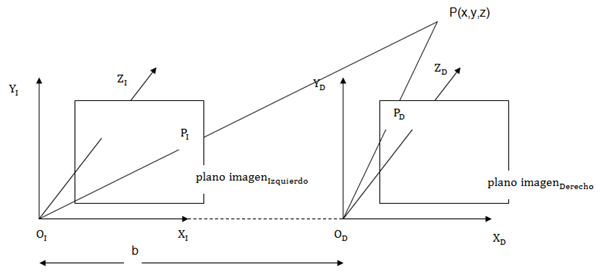
\includegraphics[width=0.5\textwidth]{./Cap6_reconstruccion/stereo.PNG}
  \caption{}
  \label{fig:Stereo}
\end{figure}

\subsection{Luz estructurada}

El método basado en la técnica de luz estructurada consiste en proyectar distintos patrones sobre la superficie a modelar que son capturadas por una cámara. Analizando las deformaciones de los patrones proyectados se obtiene información tridimensional de la posición, orientación y textura de la superficie\cite{SLightPatterns}.
Los patrones proyectados en esta técnica son variados y se clasifican en cuatro tipos: punto (\emph{singled scanned dot}), línea (\emph{slit line}), grilla (\emph{grid}) y matriz de puntos (\emph{dot matrix}).
Dependiendo del tipo de objeto y superficie a escanear pueden ocurrir problemas de oclusión, baja reflexión y puntos reflejados fuera del alcance de la cámara. Como consecuencia, existen pérdidas de puntos proyectados que no tienen proyección en el plano imagen.
Estos problemas se pueden solucionar utilizando patrones codificados adecuados. Se distinguen tres grupos de patrones clasificados: dependencia temporal, propiedades de la luz proyectada y discontinuidad de profundidad de la superficie proyectada\cite{SLightCorrespondence}.
\begin{itemize}
   \item Dependencia  temporal:
   \begin{itemize}
	\item Estática: el patrón es limitado para escenas estáticas y son necesarias proyecciones de varios patrones distintos. El movimiento de cualquier objeto de la escena mientras se realiza la obtención de los patrones proyectados producirá un error de correspondencia.
	\item Dinámica: los objetos en la escena se pueden mover y se utiliza un único patrón de proyección.
   \end{itemize}
   \item Propiedades de la luz proyectada:
   \begin{itemize}
	\item Binaria: cada uno de los puntos del patrón tiene dos posibles valores codificados con 0 y 1 respectivamente. Este valor representa opacidad y transparencia, ausencia o presencia de la luz proyectada en el objeto.
	\item Escala de grises: cada punto del patrón tiene asociado un valor de gris que representa el nivel de trasparencia o nivel de opacidad del punto para la luz proyectada. Son necesarios dos pasos, primero se obtiene una imagen de la escena iluminada con la misma luz, o sea, sin variar la intensidad. Luego, se obtiene la referencia de luz necesaria para cancelar el efecto de reflejo de la superficie que dependerá del tipo de superficie. La necesidad de estos dos pasos contribuye a que este patrón también sea clasificado como estático.
	\item Color: cada punto del patrón es asociado con un valor de tono debiendo estos ser bien diferenciados para alcanzar una segmentación eficiente. Este tipo de patrones son limitados por el color de la escena. Si presenta objetos de colores altamente saturados se producen pérdidas de regiones en el paso de segmentación que luego provoca errores en la decodificación.
   \end{itemize}
   \item Discontinuidad en profundidad de la superficie proyectada:
   \begin{itemize}
	\item Periódica: la codificación se repite periódicamente a lo largo del patrón. Esta técnica se utiliza para reducir el número de bits que codifican el patrón. Como limitante, la profundidad del objeto no puede ser mayor que la mitad de la longitud del período.%?%
	\item Absoluta: cada columna o fila del patrón proyectado tiene una única codificación. No sufre dependencia de discontinuidad de profundidad.
   \end{itemize}
\end{itemize}

\subsection{Kinect}

\emph{Kinect} es un dispositivo que se puede adicionar a la consola \emph{Xbox360} de \emph{Microsoft}. El objetivo de este dispositivo es permitir que el usuario interactúe con la consola utilizando solo el movimiento de su cuerpo. Para lograr esto, \emph{Kinect} aplica distintas técnicas de procesamiento de imágenes, considerando ubicaciones, posturas y distancias. El \emph{hardware} de \emph{Kinect} no consiste tan solo de una cámara, sino que tiene adicionalmente un emisor de infrarrojos que en base a la deformación del haz de luz determina la distancia de cada punto de la imagen capturada. Posteriormente, combina la información visual para tener una noción bastante precisa de los movimientos del usuario. A mediados del 2011 fue presentada una interfaz de programación gratuita que permite utilizar \emph{Kinect} de forma directa en aplicaciones no licenciadas para diferentes propósitos, no solo el de los videojuegos.

\begin{figure}[H]
  \centering
    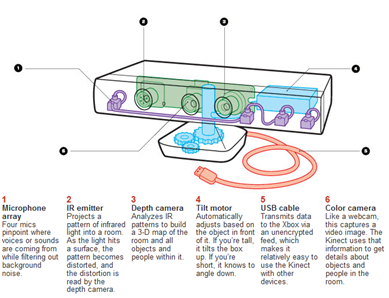
\includegraphics[width=0.5\textwidth]{./Cap6_reconstruccion/kinect.PNG}
  \caption{Componentes de un sensor Kinect}
  \label{fig:Kinect}
\end{figure}

Para el análisis de las deformaciones de los rayos y construir el mapa de profundidad, \emph{Kinect} utiliza la previamente mencionada técnica de luz estructurada. Mediante el emisor infrarrojo con el que viene equipado, se proyectan los patrones de luz por toda la escena y utilizando la cámara de profundidad se analizan las distorsiones.
También se cuenta con una cámara convencional para analizar objetos o personas en la escena y la detección de colores.
En cuanto a los usos específicos orientados a la reconstrucción tridimensional de objetos, el proyecto \emph{KinectFusion}\cite{KinectFusion}, actualmente patrocinado por \emph{Microsoft}, logra muy buenos resultados.%extender kinectfusion%

\section{Procesamiento de nube de puntos}

Al utilizar técnicas de obtención de geometría lo que se obtiene son nubes de puntos. Es necesario simplificar este modelo con el objetivo de eliminar redundancia y aumentar la velocidad en el procesamiento de los datos. Un problema adicional al volumen de la información obtenida es que comúnmente se introduce información errónea. Para solucionar este problema se realiza un suavizado en el procesamiento de la nube de puntos\cite{PCloudSimplify}.

Las heurísticas utilizadas se pueden clasificar como\cite{PntCloud}:
\begin{itemize}
   \item \emph{Clustering methods}: consta en obtener grupos de la nube de puntos en donde cada grupo se remplaza por un conjunto de puntos representativos en él. Los grupos se pueden construir utilizando un enfoque incremental en el cuál estos son creados iniciando por un punto aleatorio y agregando puntos vecinos hasta llegar a una cantidad establecida de elementos o un enfoque jerárquico en donde se particiona el conjunto de puntos recursivamente hasta conseguir grupos de un tamaño predefinido.
   \item \emph{Iterative simplification}: se recorren iterativamente los puntos de la nube contrayendo parejas en un único punto. Se evalúa el error introducido, utilizando mínimos cuadrados, que se genera en la contracción comparándolo con el error que se obtendría al contraerse con otro punto vecino eligiendo la contracción que introduce menor error al sistema. La simplificación se da por finalizada por haber logrado la cantidad de puntos deseada o por superar una cota de error a introducir en el sistema.
   \item \emph{Particle simulation}: se generan nuevos puntos que sustituyen la nube de puntos original. Se generan conjuntos de partículas que se mueven aleatoriamente en la superficie hasta lograr un balance. %Luego, utilizando el algoritmo de point–repulsion se definen en las zonas que hay mayor colisiones.%
\end{itemize}

Luego de simplificar la nube de puntos se construye un modelo tridimensional a partir de ella utilizando mallas de triángulos. La razón principal es la simplicidad de los algoritmos que dibujan triángulos. Esto permite que sean implementados fácilmente en hardware además del beneficio de que cualquier polígono con más de tres caras puede representarse como un conjunto de triángulos\cite{PCloudTriangle}.

\section{Tratamiento de malla}

Los dispositivos de captura de información tridimensional estudiados entregan la información en forma de nube de puntos. Es por ello que previo a la manipulación de la información tridimensional, es necesario procesar dicha nube de puntos para convertirla a representaciones más manejables como por ejemplo mallas triangulares.
Un algoritmo de procesamiento de malla se basa en tomar como entrada una nube de puntos, realizar un sub-muestreo y suavizado de la misma, calcular las normales en cada punto de la nube y finalmente, aplicar algoritmos de reconstrucción de malla. Esto ha sido estudiado e implementado en las bibliotecas \emph{VcgLib}\cite{VCGLib} y \emph{CGAL}\cite{CGAL}.

\begin{figure}[H]
  \centering
    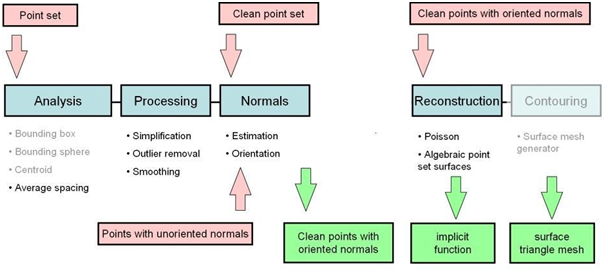
\includegraphics[width=0.5\textwidth]{./Cap6_reconstruccion/malla-flow.png}
  \caption{Típico flujo para el procesamiento de nubes de puntos. Fuente: \emph{CGAL}}
  \label{fig:Mesh-CGAL}
\end{figure}

Para la implementación de este módulo se utilizan algoritmos incluidos en \emph{VcgLib}. Para visualizar y evaluar los resultados esperados fue utilizada la aplicación de código abierto para la manipulación de mallas tridimensionales en diferentes formatos \emph{MeshLab}\cite{MeshLab}. Particularmente se utilizan los algoritmos de muestreo \emph{Poisson-disk} para reducir y normalizar los puntos de la malla inicial, \emph{normal extrapolation} para el cálculo de normales y reconstrucción de superficies de Poisson para la reconstrucción de la malla final.

\subsection{Muestreo \emph{Poisson-disk}}

El muestreo de variables aleatorias es una técnica utilizada para una gran variedad de aplicaciones como procesamiento de imágenes y geometrías. Particularmente, el muestreo \emph{Poisson-disk} se utiliza para la ubicación aleatoria de objetos en mundos artificiales, algoritmos de texturas procedurales y procesamiento de geometrías o mallas.%REFERENCIAR%
Esta técnica genera conjuntos de puntos con la propiedad de obtener puntos suficientemente juntos pero con la restricción de no estar más próximos unos de otros que una distancia mínima $R$ predeterminada.

\begin{figure}[H]
  \centering
    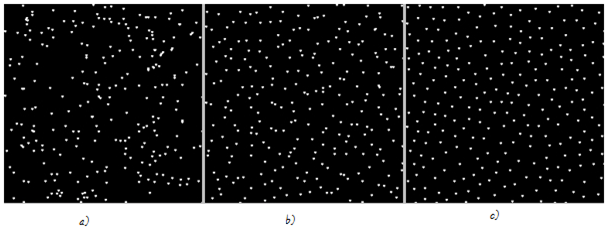
\includegraphics[width=0.5\textwidth]{./Cap6_reconstruccion/malla-poisson.png}
  \caption{a) Posición $x$ e $y$ generadas aleatoriamente. b) Imagen dividida en celdas. Puntos aleatorios generados en cada celda. c) Muestreo \emph{Poisson-disk} en dos dimensiones.}
  \label{fig:Mesh-Poisson}
\end{figure}

En líneas generales, este algoritmo genera puntos alrededor de los ya existentes en la muestra y valida si pueden ser agregados al conjunto final en caso de no violar la regla de la mínima distancia a los vecinos. Se genera una grilla en dos o tres dimensiones, dependiendo del escenario de aplicación, en la cuál cada celda contendrá al final del proceso a lo sumo un punto. Una grilla adicional es utilizada para realizar búsquedas rápidas y dos conjuntos de puntos son mantenidos durante el procesamiento para poder diferenciar los que han sido generados y los que aún necesitan procesamiento.
La implementación realizada en \emph{VcgLib} recibe tres parámetros:
\begin{itemize}
	\item 1) La cantidad de puntos en la muestra. En este caso el radio de cercanía es calculado en base a este parámetro.
	\item 2) El radio, que es a su vez utilizado para calcular el tamaño de la muestra óptimo en base a la malla inicial.
	\item 3) Sub muestreo: indica si la muestra de Poisson es un subconjunto de la muestra inicial o si se deberán generar nuevos puntos aleatoriamente.
\end{itemize}

\begin{figure}[H]
  \centering
    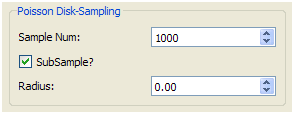
\includegraphics[width=0.5\textwidth]{./Cap6_reconstruccion/malla-poissongui.png}
  \caption{Configuración de parámetros del algoritmo \emph{Poisson-disk}}
  \label{fig:Mesh-PoissonGui}
\end{figure}

\subsection{Reconstrucción de normales}

Este algoritmo computa las normales en cada elemento de un conjunto de puntos sin la necesidad de explorar la conectividad de los triángulos. Por ello es muy útil para objetos tridimensionales sin información de caras.
Se detalla un pseudo-código del método:

%Figura: planos tangentes%

\subsubsection{Paso 1: identificar los planos tangentes para aproximar localmente la superficie y estimar así los vectores normales.}
Para cada vértice:
	\begin{itemize}
		\item Calcular el centro geométrico del plano tangente en el punto como el promedio de los $K$ puntos más cercanos.
		\item Calcular la normal asociada al centro geométrico. Se utiliza la matriz de covarianza en el punto, contemplando los mismos $K$ vecinos más cercanos de la muestra y los valores y vectores propios de la matriz de covarianza. Finalmente, ordenando los vectores propios, la estimación del vector perpendicular corresponde al vector propio de menor valor. Este método es conocido como \emph{Principal Component Analysis (PCA)}\footnote{PCA}.
	\end{itemize}

\subsubsection{Paso 2: construir un grafo en donde cada punto está conectado a los $K$ vecinos más cercanos (grafo de Riemannian)}
Se crea un grafo en cuyos nodos se guardan todas las aristas incidentes a los $K$ vecinos más cercanos. A cada arista se le asigna un peso igual al valor absoluto del producto escalar de la normal en el punto con la normal en cada uno de los $K$ vecinos:
   $$fabs(nodoActual->normal . K\_Vecinos[n]->normal)$$
\subsubsection{Paso 3: calcular el árbol de expansión mínimo sobre el grafo de Riemannian y recorrerlo para orientar las normales.}
Dado un grafo conexo, no dirigido, con sus aristas con un peso asignado, se llama árbol de expansión mínimo al sub-grafo con forma de árbol que conecta todos los nodos con un peso total mínimo conteniendo todos los nodos del grafo inicial. El grafo de entrada es el construido en el paso anterior y se utiliza el algoritmo de Kruskal\footnote{Kruskal}, uno de los varios algoritmos que resuelven el problema de encontrar un árbol de expansión mínima de un grafo.
Una vez construido el árbol de expansión, lo único que se hace es recorrerlo en orden e invertir el sentido de los vectores normales en caso de ser necesario. La condición para efectuar dicha corrección se basa en el ángulo del nodo siendo inspeccionado en comparación a todas las direcciones de las normales de los vecinos conectados a dicho nodo.

\begin{figure}[H]
  \centering
    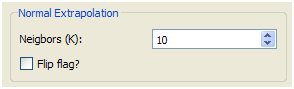
\includegraphics[width=0.5\textwidth]{./Cap6_reconstruccion/malla-normalextrapolation.png}
  \caption{Configuración de parámetros para reconstrucción de normales}
  \label{fig:Mesh-Extrapolation}
\end{figure}

\subsection{Reconstrucción de malla de Poisson}

Finalmente, para reconstruir la malla a partir de la nube de puntos y sus normales, se utiliza el algoritmo de reconstrucción de Poisson.
Se computa una función indicadora $\chi$ definida de la siguiente forma:
%Se computa una función indicadora $\chi$ en tres dimensiones definida de la siguiente forma:%

$$
\left\{ \begin{array}{rl}
 \chi = 1 & \mbox{ si puntos dentro del modelo} \\
 \chi = 0 & \mbox{ si puntos fuera del modelo}
       \end{array} \right.
$$

Luego, se obtiene una reconstrucción de la superficie mediante la extracción de la superficie de nivel en 3 dimensiones\footnote{ISO-surface} al nivel apropiado.
La estrategia se basa en la estrecha relación que hay entre los puntos de la muestra, orientados por sus normales, y la función indicadora de la muestra. Específicamente el gradiente de la función indicadora es un espacio de vectores, de valor nulo en todo el espacio excepto en puntos cercanos a la superficie, donde son iguales al vector normal a ella.
Es por eso que puntos orientados pueden ser vistos como muestras del gradiente de la función indicadora del modelo tridimensional en cuestión y es por este mismo motivo que el problema de reconstrucción de una malla puede ser visto como un problema de Poisson estándar, es decir, computar la función escalar $F$ cuya divergencia del gradiente\footnote{Laplaciano} se iguala a la divergencia del espacio de vectores de las normales.

\begin{figure}[H]
  \centering
    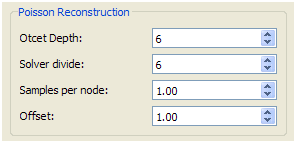
\includegraphics[width=0.5\textwidth]{./Cap6_reconstruccion/malla-poissonreconstruction.png}
  \caption{Configuración de parámetros para reconstruccion de malla de Poisson}
  \label{fig:Mesh-Normals}
\end{figure}

\subsection{Pruebas y resultados}

Para validar el correcto funcionamiento de esta técnica mediante los tres algoritmos descritos, fue utilizada una malla inicial de 5021 vértices y 9608 caras triangulares. Cabe destacar que si bien se ha mencionado que la malla de entrada debe ser simplemente una nube de puntos, se pueden utilizar mallas con caras, solo que estas serán ignoradas e incluso eliminadas de la malla de salida del primer paso del procesamiento (muestreo de \emph{Poisson-disk}).
Luego de experimentar con varios juegos de datos iniciales durante varias ejecuciones del procesamiento, se fijaron de manera personalizada para la malla de entrada algunos parámetros clave. Dado que la muestra inicial tiene alrededor de cinco mil puntos, fueron elegidas cinco mil muestras para el algoritmo de \emph{Poisson-disk}. Luego, para la extrapolación de normales se utilizan $K=15$ vecinos para la toma de decisiones locales de aproximación.
La aplicación de estos algoritmos resultó ser lo esperado en términos estructurales de cada malla procesada en cada uno de los pasos.
%Puede ir a trabajo futuro: No se llegó a procesar mallas de ambientes tridimensionales escaneados para luego ser mapeados con la herramienta.%

\begin{table}
\begin{center}
\begin{tabular}{|l||cc|} \hline
	Fase & Vértices & Caras \\
	Nube inicial & 5021 & 9608 \\
	Poisson-disk & 1776 & 0 \\
	Extrapolación Normales & 1776 & 0 \\
	Reconstrucción de Poisson & 1959 & 3910 \\ \hline %hay 1959 puntos en lugar de 1776, por que?%
\end{tabular}
\caption{Comparación de estructura de mallas de entrada y salida en cada fase}
\end{center}
\end{table}

\begin{figure}[H]
  \centering
    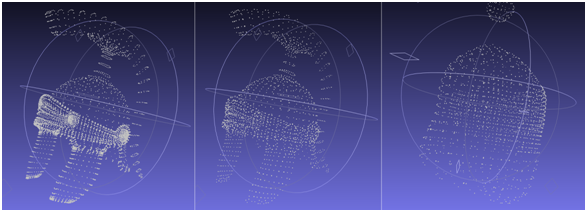
\includegraphics[width=0.8\textwidth]{./Cap6_reconstruccion/malla-nubepuntos.png}
  \caption{1) Nube de puntos inicial con 5021 vértices. 2) Resultado de muestreo \emph{Poisson-disk} con 1776 vértices. 3) Luego de extrapolar normales y reconstruir la malla con 1959 vértices y 3910 caras.}
  \label{fig:Mesh-Results}
\end{figure}
 
%Se observaron buenos tiempos computacionales de respuesta. Si bien la malla utilizada no es de un tamaño considerable, estamos hablando de algoritmos de orden relativamente alto.%
